\chapter{The Information Bottleneck Principle}
\label{chap:information_bottleneck}

% 1. Descriptive
\section{The Quest for Minimal Sufficient Representations}

In the paradigm of deep learning, we often construct layered transformations of high-dimensional inputs---such as images, text, or audio---into increasingly abstract representations. At its core, this process is an exercise in distillation. When classifying an image of a dog, the neural network does not need to memorize the exact lighting conditions, the background foliage, or the precise orientation of every strand of fur. Instead, it must extract only those features that are relevant to the label ``dog'' while discarding everything else. 

This intuitive notion of discarding irrelevant information while preserving task-relevant information is mathematically formalized by the \textit{Information Bottleneck (IB) principle}, first introduced by Naftali Tishby, Fernando Pereira, and William Bialek in 1999. The IB principle asserts that an optimal representation is one that maximally compresses the input data while retaining as much information as possible about the desired target variable. It frames learning not merely as minimizing an error on a dataset, but as solving a fundamental trade-off between compression (forgetting) and prediction (remembering).

Consider an analogy: writing a summary of a dense, 500-page historical biography. If you simply copy the entire book verbatim, you retain 100\% of the relevant historical facts, but your summary is utterly uncompressed and perhaps useless for a quick review. Conversely, if you write a single sentence---"A person lived and died."---you have achieved maximum compression, but you have lost almost all relevant details. The ideal summary sits delicately on the frontier between these two extremes, selectively filtering out the noise (the day-to-day minutiae) to preserve the signal (the overarching historical impact). 

In deep learning, the input space $\mathcal{X}$ is often vast and highly redundant. A neural network $f_\theta$ processes an input $x \in \mathcal{X}$ to form a latent representation $z$. To make accurate predictions about a target $y \in \mathcal{Y}$, $z$ must contain information about $y$. The Information Bottleneck provides a principled, information-theoretic loss function to explicitly seek this optimal $z$. It defines a strictly quantitative metric for what makes a representation ``good,'' allowing us to analyze learning dynamics and generalization without relying exclusively on the empirical loss.

\section{The Mathematical Framework}

\subsection{The Information Bottleneck Lagrangian}

Let $X$ denote the random variable representing the input data, $Y$ the target variable (e.g., labels), and $Z$ the learned representation. Since the representation is generated exclusively from the input data, the variables naturally form the Markov chain $Y \leftrightarrow X \leftrightarrow Z$. This implies that conditionally on $X$, $Z$ is independent of $Y$; or equivalently, $p(y, z | x) = p(y|x)p(z|x)$. The representation $Z$ has no independent access to $Y$ other than what it can glean through $X$.

\begin{figure}[htbp]
    \centering
    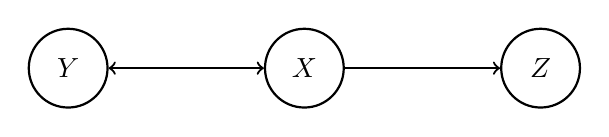
\begin{tikzpicture}[node distance=2cm, thick,
        every node/.style={circle, draw, minimum size=1cm, align=center}]
        \node (Y) {$Y$};
        \node (X) [right of=Y, node distance=3cm] {$X$};
        \node (Z) [right of=X, node distance=3cm] {$Z$};
        
        \draw[<->] (Y) -- (X);
        \draw[->] (X) -- (Z);
    \end{tikzpicture}
    \caption{The Information Bottleneck Markov Chain. The representation $Z$ depends on the target $Y$ only through the input data $X$.}
    \label{fig:ib_markov}
\end{figure}

The objective of the Information Bottleneck is to find a stochastic mapping $p(z|x)$ that minimizes the mutual information between the input and the representation, $I(X; Z)$, subject to the constraint that the mutual information between the representation and the target, $I(Z; Y)$, is greater than or equal to some threshold $I_c$. 

Using the method of Lagrange multipliers, we can formulate this as an unconstrained optimization problem. We seek to minimize the Information Bottleneck Lagrangian, defined as:
\begin{equation}
    \mathcal{L}_{\text{IB}}[p(z|x)] = I(X; Z) - \beta I(Z; Y)
\end{equation}
where $\beta \in [0, \infty)$ is a trade-off parameter that controls the relative importance of prediction versus compression.
\begin{itemize}
    \item As $\beta \to 0$, the penalty on $I(Z; Y)$ vanishes, and the optimal solution is to compress entirely, driving $I(X; Z) \to 0$ (yielding a representation completely independent of the input, and thus useless for predicting $Y$).
    \item As $\beta \to \infty$, the focus shifts entirely to maximizing $I(Z; Y)$, essentially demanding sufficient statistics of $X$ for $Y$, with no regard for the complexity or size of the representation.
\end{itemize}

\begin{theorem}[Data Processing Inequality Bounds]
    For the Markov chain $Y \leftrightarrow X \leftrightarrow Z$, the mutual information between the representation and the target is strictly bounded by the mutual information between the input and the target:
    \begin{equation}
        I(Z; Y) \le I(X; Y)
    \end{equation}
\end{theorem}
\begin{proof}
    By the chain rule for mutual information, we can expand $I(X, Z; Y)$ in two ways:
    \begin{align}
        I(X, Z; Y) &= I(Z; Y) + I(X; Y | Z) \\
        I(X, Z; Y) &= I(X; Y) + I(Z; Y | X)
    \end{align}
    Because $Y \leftrightarrow X \leftrightarrow Z$ forms a Markov chain, $Z$ and $Y$ are conditionally independent given $X$, meaning $I(Z; Y | X) = 0$. Equating the two expansions yields:
    \begin{equation}
        I(Z; Y) + I(X; Y | Z) = I(X; Y)
    \end{equation}
    Since conditional mutual information is non-negative ($I(X; Y | Z) \ge 0$), it immediately follows that $I(Z; Y) \le I(X; Y)$. 
\end{proof}
This theorem reinforces that no representation $Z$ can ever contain more information about $Y$ than was originally present in $X$.

\subsection{Exact Solutions and Self-Consistent Equations}

For discrete probability spaces, we can derive the exact functional form of the optimal mapping $p(z|x)$ that minimizes $\mathcal{L}_{\text{IB}}$.

\begin{theorem}[IB Self-Consistent Equations]
    \label{thm:ib_equations}
    The stochastic mapping $p(z|x)$ that minimizes the Information Bottleneck Lagrangian $\mathcal{L}_{\text{IB}} = I(X; Z) - \beta I(Z; Y)$ satisfies the self-consistent equation:
    \begin{equation}
        p(z|x) = \frac{p(z)}{Z(x, \beta)} \exp\left(-\beta D_{\text{KL}}(p(y|x) \parallel p(y|z))\right)
    \end{equation}
    where $Z(x, \beta)$ is a normalization constant for each $x$.
\end{theorem}

\begin{proof}
    We wish to minimize $\mathcal{L}_{\text{IB}}$ with respect to the conditional distribution $p(z|x)$. The mutual information terms are:
    \begin{align}
        I(X; Z) &= \sum_{x,z} p(x) p(z|x) \log \frac{p(z|x)}{p(z)} \\
        I(Z; Y) &= \sum_{y,z} p(y,z) \log \frac{p(y|z)}{p(y)}
    \end{align}
    Note that by the Markov property, $p(y, z) = \sum_x p(x, y, z) = \sum_x p(x) p(y|x) p(z|x)$. 
    To enforce the constraint that $\sum_z p(z|x) = 1$ for all $x$, we introduce Lagrange multipliers $\lambda(x)$. The extended Lagrangian is:
    \begin{equation}
        \tilde{\mathcal{L}} = I(X; Z) - \beta I(Z; Y) - \sum_x \lambda(x) \left( \sum_z p(z|x) - 1 \right)
    \end{equation}
    Taking the variational derivative with respect to $p(z|x)$ yields:
    \begin{equation}
        \frac{\delta \tilde{\mathcal{L}}}{\delta p(z|x)} = p(x) \left( \log \frac{p(z|x)}{p(z)} + 1 - 1 \right) - \beta p(x) \sum_y p(y|x) \left( \log \frac{p(y|z)}{p(y)} + 1 - 1 \right) - \lambda(x) = 0
    \end{equation}
    (We omit the detailed proof that variations involving $p(z)$ and $p(y|z)$ cancel out, which relies on them being marginals of $p(z|x)$). Dividing by $p(x)$ and rearranging gives:
    \begin{equation}
        \log p(z|x) = \log p(z) + \beta \sum_y p(y|x) \log \frac{p(y|z)}{p(y)} + \frac{\lambda(x)}{p(x)}
    \end{equation}
    We can add and subtract $\beta \sum_y p(y|x) \log p(y|x)$ to form a Kullback-Leibler divergence:
    \begin{align*}
        \log p(z|x) &= \log p(z) - \beta \sum_y p(y|x) \log \frac{p(y|x)}{p(y|z)} + \beta \sum_y p(y|x) \log \frac{p(y|x)}{p(y)} + \frac{\lambda(x)}{p(x)} \\
        &= \log p(z) - \beta D_{\text{KL}}(p(y|x) \parallel p(y|z)) + C(x, \beta)
    \end{align*}
    Exponentiating both sides, we absorb the term $C(x, \beta)$, which only depends on $x$, into a normalization partition function $Z(x, \beta)$:
    \begin{equation}
        p(z|x) = \frac{p(z)}{Z(x, \beta)} \exp\left(-\beta D_{\text{KL}}(p(y|x) \parallel p(y|z))\right)
    \end{equation}
\end{proof}

This elegantly shows that the optimal probability of mapping $x$ to $z$ decays exponentially with the KL divergence between the true label distribution $p(y|x)$ and the label distribution predicted from the latent representation $p(y|z)$. The representation must reflect the true conditional distribution of the labels as closely as possible, weighted by the severity of the $\beta$ parameter.

\subsection{The Information Plane}

By plotting $I(X; Z)$ on the horizontal axis and $I(Z; Y)$ on the vertical axis, we construct the \textit{Information Plane}. For a given dataset, mapping the optimal values of $I(Z;Y)$ against a constraint on $I(X;Z)$ yields a monotonic, concave function known as the IB bound.

\begin{figure}[htbp]
    \centering
    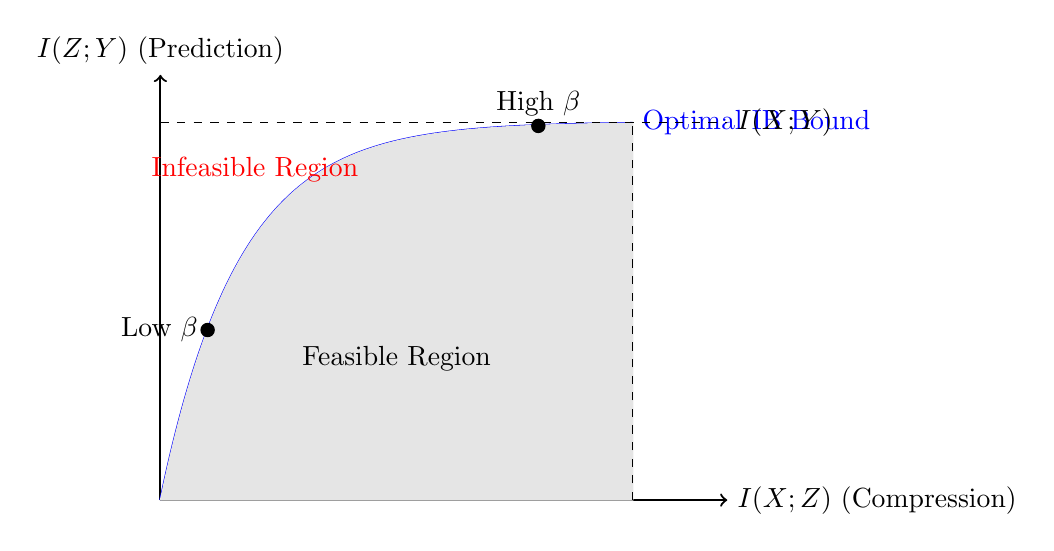
\begin{tikzpicture}[scale=1.2]
        % Axes
        \draw[->, thick] (0,0) -- (6,0) node[right] {$I(X; Z)$ (Compression)};
        \draw[->, thick] (0,0) -- (0,4.5) node[above] {$I(Z; Y)$ (Prediction)};
        
        % IB Bound Curve
        \draw[thick, blue, domain=0:5, smooth, samples=100] plot ({\x}, {4*(1 - exp(-1.2*\x))});
        
        % Labels
        \node[blue, right] at (5, 4.0) {Optimal IB Bound};
        \filldraw[gray!20] (0,0) -- plot[domain=0:5, smooth, samples=100] ({\x}, {4*(1 - exp(-1.2*\x))}) -- (5,0) -- cycle;
        \node at (2.5, 1.5) {Feasible Region};
        \node[red] at (1.0, 3.5) {Infeasible Region};
        
        % Data processing limits
        \draw[dashed] (0,4) -- (6,4) node[right] {$I(X; Y)$};
        \draw[dashed] (5,0) -- (5,4);
        
        % Points on curve
        \filldraw[black] (4, 3.96) circle (2pt) node[above] {High $\beta$};
        \filldraw[black] (0.5, 1.8) circle (2pt) node[left] {Low $\beta$};
        
    \end{tikzpicture}
    \caption{The Information Plane. The theoretical bound defines the maximum mutual information $I(Z;Y)$ achievable for a given constraint on $I(X;Z)$. Points above the blue curve are strictly infeasible by the Data Processing Inequality and the Information Bottleneck principle.}
    \label{fig:info_plane}
\end{figure}

The Information Plane allows us to track the state of a neural network layer-by-layer or epoch-by-epoch. In this plane, any given deterministic or stochastic function $Z = f(X)$ forms a single point. 

\subsection{A Numerical Example: The Binary Symmetric Channel}

To solidify these concepts, consider a simple numerical example. Suppose our target variable $Y$ is a uniform binary variable, $Y \in \{0, 1\}$. Our input data $X$ is generated by passing $Y$ through a Binary Symmetric Channel (BSC) with crossover probability $p = 0.1$. This means $P(X \neq Y) = 0.1$. 

We want to learn a compressed binary representation $Z \in \{0, 1\}$. We parameterize the stochastic encoder symmetrically: let $P(Z=0 | X=0) = q$ and $P(Z=1 | X=1) = q$. By symmetry, $P(Z=1) = P(Z=0) = 0.5$.

We can compute the mutual information $I(X; Z)$:
\begin{equation}
    I(X; Z) = H(Z) - H(Z|X) = 1 - H(q)
\end{equation}
where $H(q) = -q \log_2(q) - (1-q) \log_2(1-q)$ is the binary entropy function. 

To compute $I(Z; Y)$, we must find the effective crossover probability between $Y$ and $Z$. A bit is flipped between $Y$ and $Z$ if it is flipped in the transition $Y \to X$ but not in $X \to Z$, or if it is not flipped in $Y \to X$ but is flipped in $X \to Z$. Thus, the effective error probability is:
\begin{equation}
    \alpha \equiv P(Z \neq Y) = p \cdot q + (1-p) \cdot (1-q)
\end{equation}
Then, the mutual information is:
\begin{equation}
    I(Z; Y) = H(Z) - H(Z|Y) = 1 - H(\alpha)
\end{equation}
By sweeping the parameter $q \in [0.5, 1.0]$, we systematically traverse the feasible region in the information plane for this specific architecture. For $q=1$ (a deterministic mapping $Z=X$), we have $I(X;Z) = 1$ bit, and $I(Z;Y) = 1 - H(0.1) \approx 0.531$ bits. For $q=0.5$ (a completely random mapping), we have $I(X;Z) = 0$ bits, and $I(Z;Y) = 0$ bits. Intermediate values of $q$ interpolate between these extremes, tracing out the optimal curve governed by the Lagrangian mapping dictated by $\beta$.

\begin{horizon}
The mathematical foundations of the Information Bottleneck are rigorous and exact for discrete spaces and specific continuous cases like jointly Gaussian variables. However, the exact application of the IB principle to the dynamics of deep neural networks remains highly debated.

It is conjectured by Tishby and others that Stochastic Gradient Descent (SGD) in deep neural networks implicitly solves the IB problem. This hypothesis suggests that training naturally bifurcates into two distinct phases: a rapid "fitting phase" where layers quickly increase $I(Z; Y)$ while also increasing $I(X; Z)$, followed by a much longer "compression phase" where $I(Z; Y)$ remains roughly constant while the network actively sheds irrelevant information, driving $I(X; Z)$ down. 

An open question is whether this compression phase is a universal property of learning or an artifact of specific choices, such as double-sided saturating activation functions (like $\tanh$). Evidence suggests that networks using strictly monotonic, non-saturating functions like ReLU may not exhibit obvious compression in $I(X; Z)$ when measured via continuous differential entropy, because continuous bijections inherently preserve mutual information. Future work might show whether redefining mutual information in terms of robust geometric measures or noisy activations can mathematically bridge the gap between empirical deep learning success and the Information Bottleneck bound.
\end{horizon}

\section{Summary}

In this chapter, we formalized the Information Bottleneck principle as a foundational method for evaluating the quality of representations. By framing learning as an explicit optimization of the trade-off between minimizing $I(X; Z)$ (compression) and maximizing $I(Z; Y)$ (prediction), we established the theoretical ceiling of performance in the Information Plane. We derived the self-consistent equations that dictate the optimal assignment of inputs to latent representations, revealing that optimal embeddings depend exponentially on the KL divergence between true and predicted label distributions. 

\section*{Exercises}

\begin{enumerate}
    \item \textbf{Gaussian Information Bottleneck:} Suppose $X, Y, Z$ are all scalar, jointly Gaussian random variables. Assume $Y \sim \mathcal{N}(0, \sigma_y^2)$ and $X = Y + \epsilon$ where $\epsilon \sim \mathcal{N}(0, \sigma_e^2)$. Derive the exact analytical formula for the optimal Information Bottleneck curve $I(Z; Y)$ as a function of $I(X; Z)$.
    \item \textbf{Limits of $\beta$:} Prove mathematically that in the strict limit as $\beta \to 0$, the optimal solution for the IB Lagrangian $\mathcal{L}_{\text{IB}}$ yields $I(X; Z) = 0$ and $p(z|x) = p(z)$ for all $x$. 
    \item \textbf{Markov Independence:} In the derivation of the Data Processing Inequality bound $I(Z; Y) \le I(X; Y)$, we relied on the Markov chain $Y \leftrightarrow X \leftrightarrow Z$. Provide a concrete, real-world scenario involving machine learning where this Markov chain assumption is violated, and explain how it affects the bounds.
    \item \textbf{Numerical Optimization:} Implement the Blahut-Arimoto algorithm in Python to empirically find the optimal $p(z|x)$ for the Binary Symmetric Channel example given in the chapter. Plot the resulting Information Plane curve for a range of $\beta \in [0.01, 100]$.
\end{enumerate}

% TODO-CITE: Ensure all named results are cited.
